
%Volume: maximaal aantal pagina van inleiding t/m literatuur, maximaal  35 bladzijden (excl.bijlagen).
\documentclass[11pt]{report}
\usepackage[a4 paper, headheight=1pt, headsep=1pt] {geometry}
\usepackage{titlesec}
\titleformat{\chapter}[display]   
{\normalfont\huge\bfseries}{\chaptertitlename\ \thechapter}{8pt}{\huge}   
\titlespacing*{\chapter}{0pt}{-65pt}{8pt}
\titlespacing*{\section}{0pt}{5pt}{1pt}
\setlength{\parindent}{0pt}
\setlength{\parskip}{5pt plus 2pt minus 1pt}
\setlength{\textheight}{680pt}
\setlength{\headsep}{0pt}
%\usepackage{showframe}
\usepackage{graphicx}
\usepackage[usenames,dvipsnames]{color}
%\usepackage{picins}
\footskip = 20pt 
\usepackage[nodayofweek]{datetime}
\usepackage{tikz}
\usepackage{todonotes}
\usetikzlibrary{shapes.geometric, arrows}
\usepackage{pdfpages}
\usepackage{xcolor}
\usepackage{siunitx}

\begin{document}
\begin{titlepage}
	\begin{center}
	\vspace*{0\textheight}
	{\scshape\LARGE Utrecht University \par}
	\vspace{1cm} 
	\line(4,0){300}
	\vspace{0.5cm} \\
	{\Large \bfseries Local characteristics of two Svalbard glaciers\\}
	\vspace{0.5cm}
	\line(4,0){300} \\

	\vspace{2.5cm}
	\begin{minipage}[t]{0.4\textwidth}
	\begin{flushleft} \large
	\emph{Author:}\\
	{Isolde Glissenaar}\\
	{Daphne van Zanten} \\
	\end{flushleft}
	\end{minipage} %No ENTER BECAUSE!
	\begin{minipage}[t]{0.4\textwidth}
	\begin{flushright} \large
	\emph{Supervisor:} \\
	{Dr. C.H. Tijm-Reijmer}\\
	\end{flushright}
	\end{minipage}\\[0.4cm]

	\vspace{3.5cm}
	\large \textit{}\\[1cm]

	{\large {\today}\\[2cm] % Date

	\noindent
	
\includegraphics[scale=1, width=0.35\textwidth]{UU-logo.jpg}}
	\end{center}
\end{titlepage}

\newpage
\tableofcontents

\chapter{Introduction}\label{sec:intro}
\pagenumbering{arabic}
\setcounter{page}{2}
%\todo{In report: \\
%- General description experiment and conditions\\
%– General description of the dataset and data handling\\
%– Detailed analyses of chosen subject\\
%+- 15 pages}

Around 1595, a Dutch man called Willem Barentsz went on expedition to the North East Passage when he discovered  Svalbard. \cite{sval} To imagine this situation, a painting of his ship is made and visible in figure \ref{fig:wbs}. From this moment, Dutch people were concerned by research on Svalbard. In 2010, people observed big climate changes, while they had less research data. To investigate the newest situation on Svalbard, SEES (Netherlands Scientific Expedition Edgeøya Spitsbergen) has been established, which is still active nowadays. \cite{sees} 

\begin{figure}[h]
\includegraphics[scale=1, width=0.5\textwidth]{wbs.jpg}
\centering{}
\caption{Ship of Willem Barentsz at the discovery of Svalbard, made by Maritim painter Arnold de Lange}
\label{fig:wbs}
\end{figure}

In this study, measurement data from Svalbard is used to answer the question:

\textit{How can the local characteristics of two Svalbard glaciers be explained?}

To investigate this, sub-questions arise:
\textit{What are the characteristics of the Nordenskiöldbreen and the Ulvebreen?} and \textit{What are the differences between the two glaciers?}

The conducted research is described comprehensively in this report. Explained in chapter \ref{sec:method} are the origin of the measurements and the method of handling obtained data,  which is used to analyze the data. Chapter \ref{sec:results} contains results of this research, obtained by comparing data. In chapter \ref{sec:discussion} results are discussed and compared with expectations. In chapter \ref{sec:conclusion}, a conclusion is presented. Finally, a bibliography is appended as well as other appendices.

\newpage

\chapter{Method}\label{sec:method}

To investigate the local characteristics of two glaciers on Svalbard, the location of the glaciers are described in section \ref{sec:loc}. On those glaciers, instruments are installed to measure different variables, which are described in section \ref{sec:instr}. Finally, the huge amount of data from those instruments has to transform into a manageable amount, which is described in chapter \ref{sec:datah}.

%\textcolor{red}{location of measurements, instruments, data handling (on making the daily averages and handling the data gaps.)} are investigated. 

\section{Location} \label{sec:loc}
\todo{bronnen}
This study discusses data from weather stations situated on Svalbard, which is a Norwegian archipelago in the Arctic Ocean, north of the European mainland. The island group ranges from 74$^\circ$N to 81$^\circ$N in latitude. The archipelago features an Arctic climate, although with higher temperatures than other areas on the same latitude.  The northernmost branch of the relatively warm North Atlantic Current, the West Spitsbergen Current (Figure \ref{fig:current}), moderates the temperature on the western side of the island. The East Spitsbergen Current brings colder water from higher latitudes to the eastern side of the archipelago. The mean temperatures range from $\SI{-16}{^\circ C}$ in February to $\SI{6}{^\circ C}$ in July (Norwegian Meteorological Institute) at Svalbard Lufthavn, in the middle of the main island Spitsbergen. The mean yearly precipitation at Svalbard Lufthavn is 190 mm. 
 

\begin{figure}[h]
\includegraphics[scale=1, width=0.5\textwidth]{currents_svalbard.jpg}
\centering{}
\caption{Map of Svalbard showing key features and major ocean currents (Storrie et al., 2018).}
\label{fig:current}
\end{figure}

All three measurement locations are situated on the largest island, called Spitsbergen. Data are used from two weather stations from the Institute for Marine and Atmospheric research Utrecht (IMAU) located on two glaciers and data from an operational station from the Norwegian Meteorological Institute (Figure \ref{fig:locations}).

\begin{figure}[h]
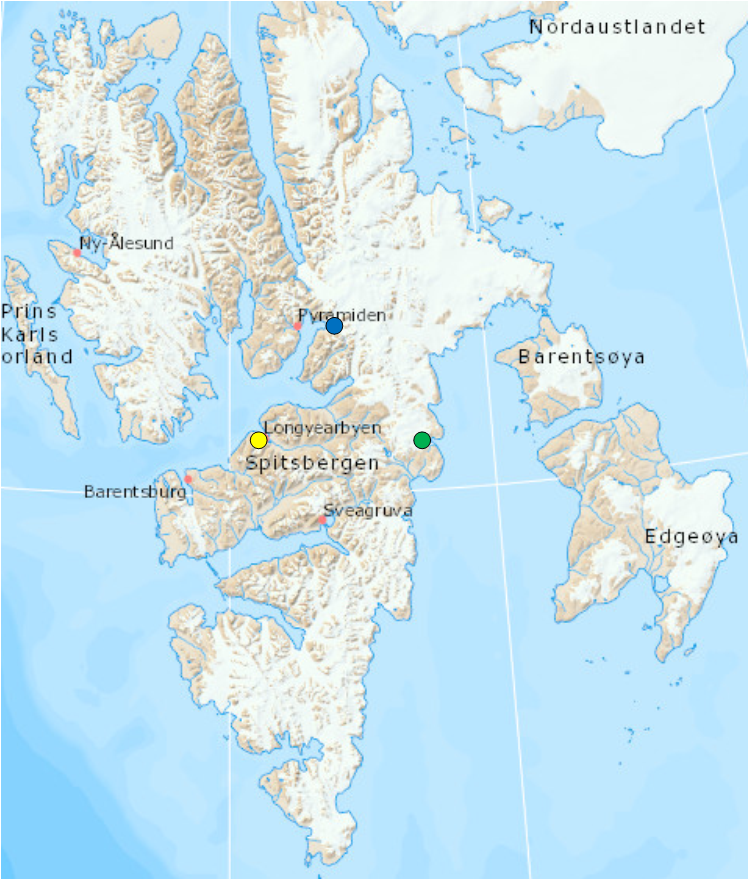
\includegraphics[scale=1, width=0.5\textwidth]{svalbard_locations.png}
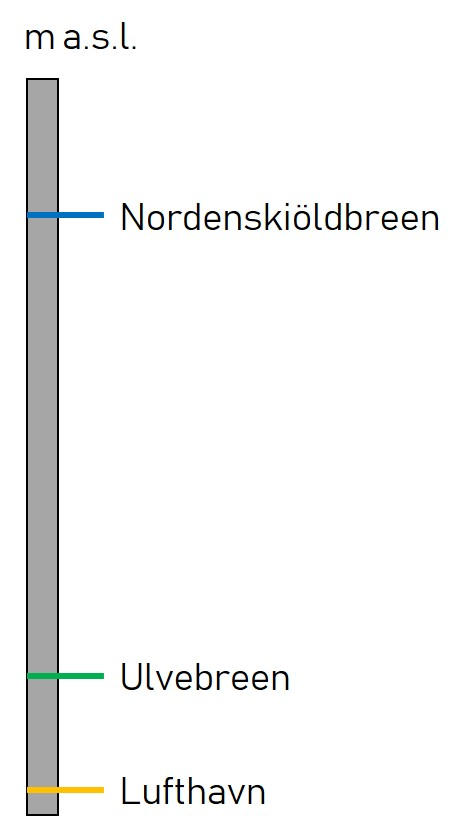
\includegraphics[scale=1, width=0.33\textwidth]{height.jpg}
\centering{}
\caption{Left: Map of Svalbard showing the locations of the weather stations. Blue: Nordenski\H{o}ldbreen, green: Ulvebreen, yellow: Svalbard Lufthavn. Right: Schematic picture of differences in height}
\label{fig:locations}
\end{figure}
\todo{Map from the Norwegian Polar Institute (toposvalbard)}

The weather stations are situated on the Nordenski\H{o}ldbreen and the Ulvebreen. The Nordenski\H{o}ldbreen is a marine-terminating glacier, terminating in Adolfsbukta, which is a branch of Billefjorden. The glacier is situated roughly in the middle of the island Spitsbergen. The glacier is $\SI{25}{km}$ long, $\SI{11}{km}$ wide and located 529 meters above sea level (m a.s.l.). It originates from Lomonosovfonna and flows in southwesterly direction (Figure \ref{fig:norden}). 

The Ulvebreen is also a marine-terminating glacier. This glacier is a tributary to Nordmannsfonna and terminates in Dunérbukta, at the east of Spitsbergen. The Ulvebreen is $\SI{9}{km}$ long, $\SI{2.5}{km}$ wide and located at 140 m a.s.l., which is a difference of 389 meter compared to the Nordenski\H{o}ldbreen. It flows in southeasterly direction (Figure \ref{fig:ulve}). 

The third measurement location is an operational station at Svalbard Lufthavn, close to the largest settlement on Svalbard: Longyearbyen. This operational station is run by the Norwegian Meteorological Institute. Svalbard Lufthavn is located at Adventfjorden, which debouches into Isfjorden at 28 m a.s.l., which is a difference of 501 meter with the Nordenski\H{o}ldbreen and 112 meter with the Ulvebreen, also schematically drawn in figure \ref{fig:locations}.

\begin{figure}[h]
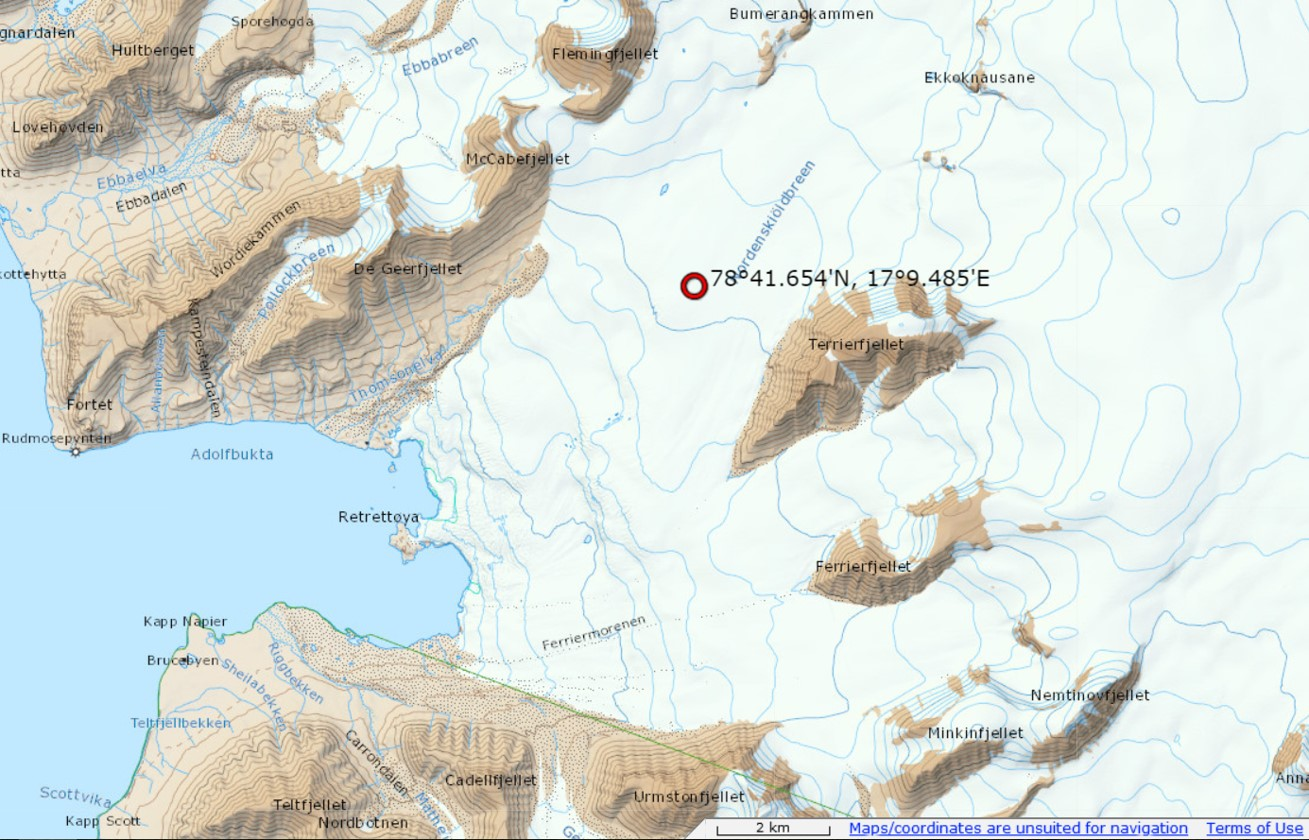
\includegraphics[scale=1, width=0.45\textwidth]{nskimap.jpg}
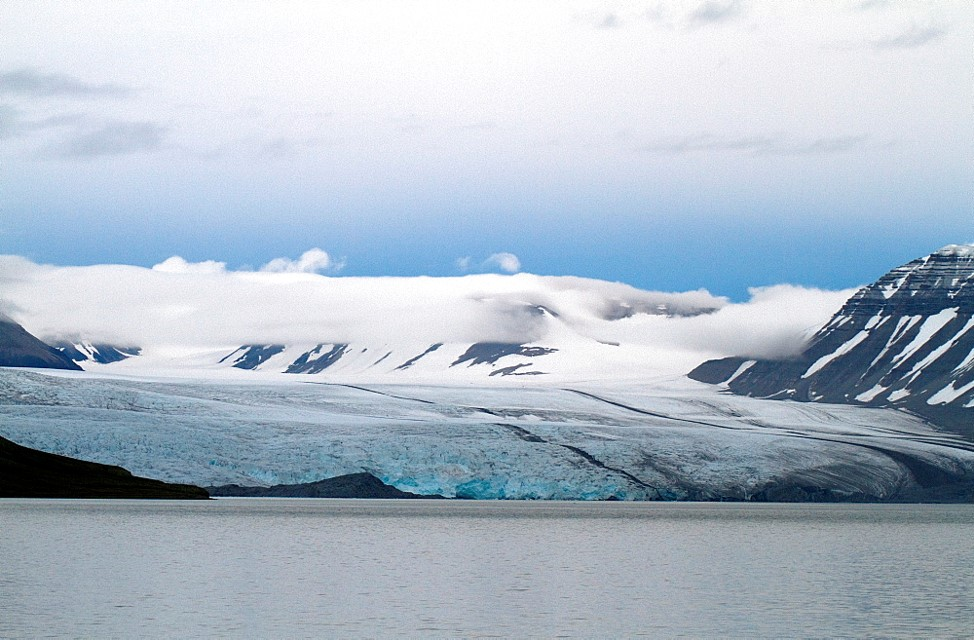
\includegraphics[scale=1, width=0.45\textwidth]{view1.jpg}
\centering{}
\caption{Left: Map showing the Nordenski\H{o}ldbreen and the location of the weather station (toposvalbard). Right: A picture of the terminus of the Nordenski\H{o}ldbreen in Adolfsbukta.}
\label{fig:norden}
\end{figure}

\begin{figure}[h]
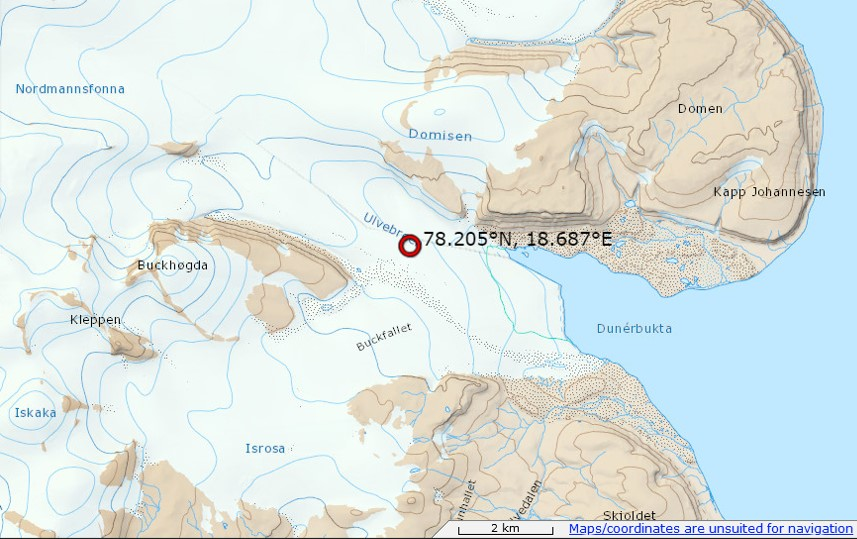
\includegraphics[scale=1, width=0.45\textwidth]{ulvemap.jpg}
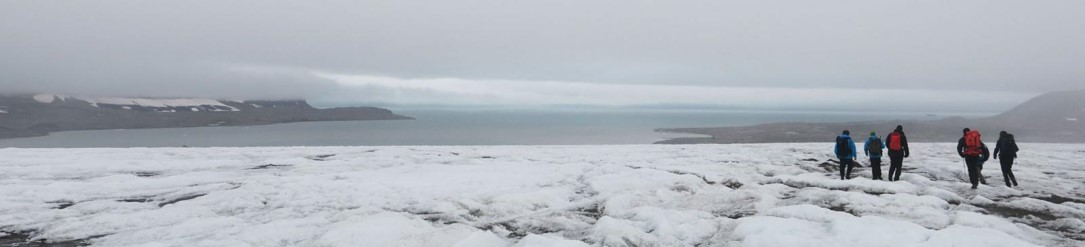
\includegraphics[scale=1, width=0.45\textwidth]{view2.jpg}
\centering{}
\caption{Left: Map showing the Ulvebreen and the location of the weather station (toposvalbard). Right: A picture made on top of the Ulvebreen (IMAU).}
\label{fig:ulve}
\end{figure}

\newpage
\section{Instruments}\label{sec:instr}
Measurement data used for this study is mainly coming from two Automatic Weather Stations (AWS) on glaciers, as visible in figure \ref{fig:instrn} for the Nordenskiolbreen and figure \ref{fig:instru} for the Ulvebreen.

\begin{figure}[h]
\raggedright
\begin{minipage}{0.5\textwidth}
\centering{}
    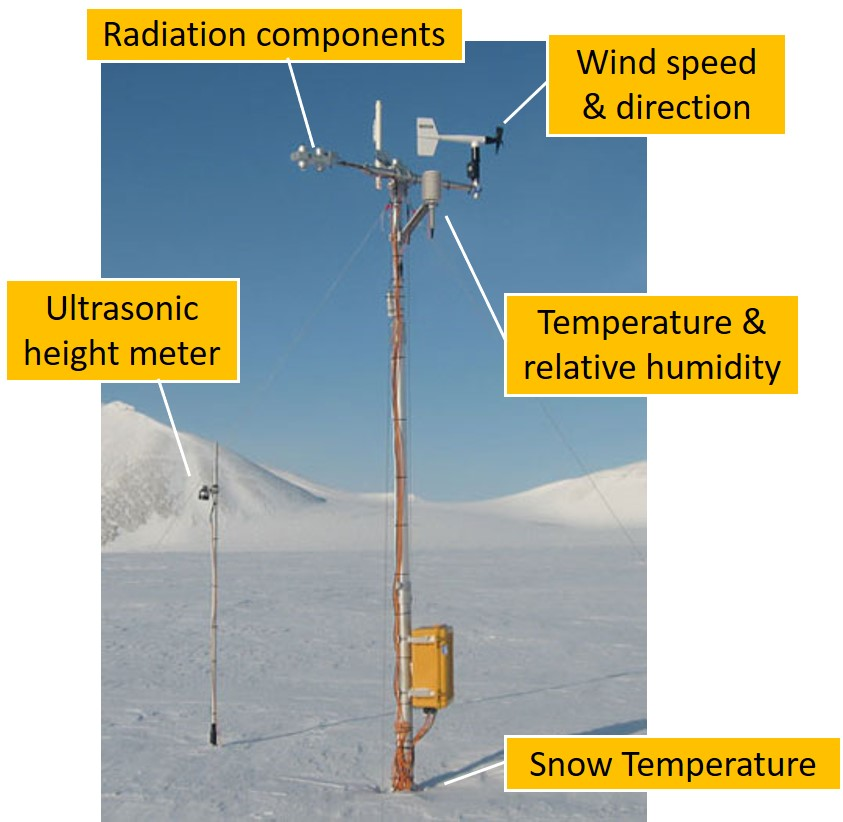
\includegraphics[width=0.95\textwidth]{nski1.jpg}
    \caption{AWS Nordenski\H{o}ldbreen \cite{uuproj}}
    \label{fig:instrn}
\end{minipage}%
\begin{minipage}{0.5\textwidth}
\centering{}
    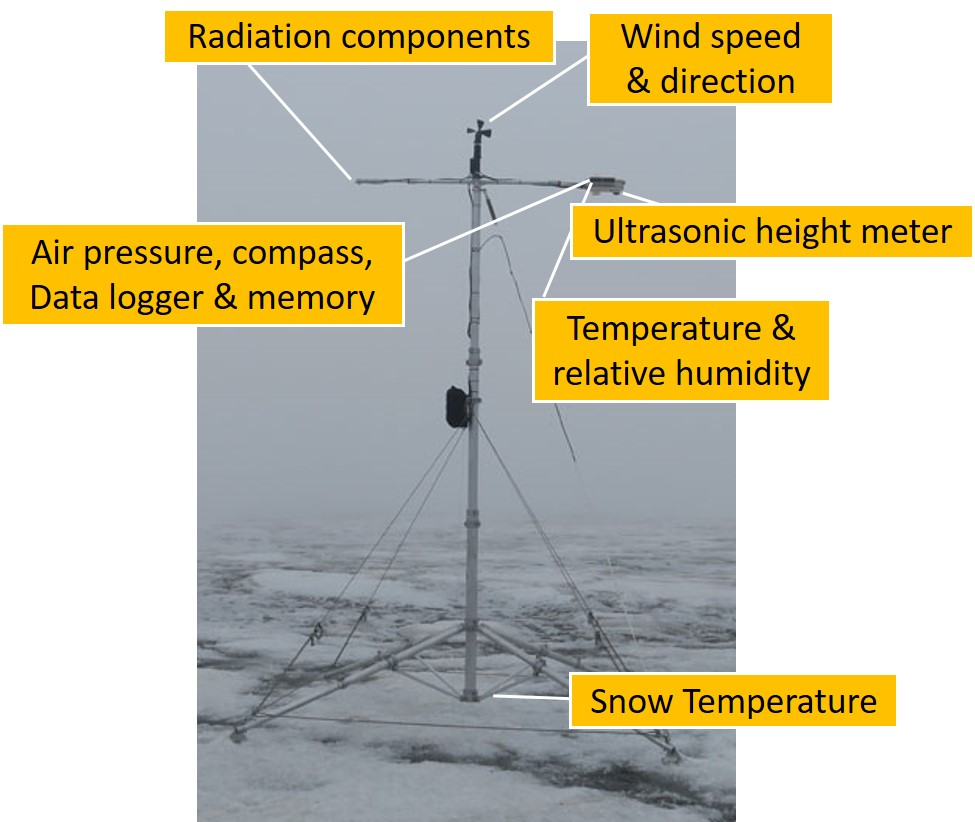
\includegraphics[width=0.95\textwidth]{ulve1.jpg}
    \caption{AWS Ulvebreen \cite{uuproj}}
    \label{fig:instru}
\end{minipage}%
\end{figure}

In figures \ref{fig:instrn} and \ref{fig:instru}, different instruments are visible, where each instrument has his own specialty. Next the different measured variables at the Nordenski\H{o}ldbreen and the Ulvebreen are roughly explained. Finally, the used measurement data of the Lufthavn is described.\\

The Nordenski\H{o}ldbreen was operational from March 2009 until 2016. Within this time, every 30 minutes measurements of different variables were saved to the logger. Unfortunately, because of broken instruments and a location which is hard to reach, the measurement data of the Nordenski\H{o}ldbreen is not serried the whole time. A inclinometer is used to measure the tilt and an anemometer is used to measure the horizontal wind speed and direction. A radiometer with two pyranometers is used to measure the shortwave and longwave radiation for incoming and outgoing directions. Thereby, the net temperature of the radiometer is measured and a barometer is measuring the pressure. The snow temperature is measured at 10 different depths. The \todo{sonic snow height} is measured twice and a quality number is used to pick a measurement (1 or 2). Finally, the battery is logged as well as the temperature in the logger, to look at the status of the instruments itself. With all those measurements, the surface temperature is derived from the outgoing longwave radiation. The Potential temperature is based on the main hut temperature and pressure. The temperature at 2 meter is based on the main hut temperature and the sonic snow height. The specific humidity is based on the main hut temperature and pressure as well. \\

The AWS on the Ulvebreen is placed as part of the Netherlands Scientific Expedition Edge$ø$ya Spitsbergen (SEES) in 2015 \cite{uuproj}. Like at the Nordenski\H{o}ldbreen, every 30 minutes data is saved to a logger and this process is still going on (also with some gaps in between). Measurements of the Ulvebreen are slightly different in some ways compared to the Nordenski\H{o}ldbreen. For example, instead of snow temperature at 10 different locations, it are 8 different locations. Also, in addition to the Nordenski\H{o}ldbreen, an ablation draw wire is added to the AWS. Figure \ref{fig:ablation} shows a schematic picture of the ablation wire. 

\begin{figure}[h]
\raggedright
\begin{minipage}{0.65\textwidth}
\raggedright
    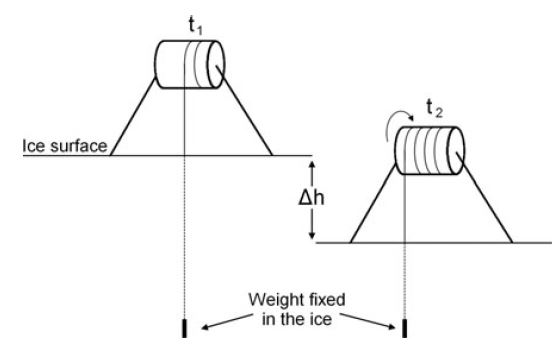
\includegraphics[scale=1, width=1\textwidth]{abliationwire.jpg}	 
    \caption{Ablation Wire \cite{abl}}
    \label{fig:ablation}
\end{minipage}%
\end{figure}

As visible in figure \ref{fig:ablation}, weights are fixed in the ice. A draw wire sensor is placed on the other side of the wire. This sensor is measuring the difference in time and the difference in height. \cite{abl} The difference in height is because of the ablation at the glacier.

Finally, from the lufthavn observation station, only data of the wind direction and wind speed, air pressure at station level and air temperature is used to compare this with the two glaciers.

\section{Data handling}\label{sec:datah}

As described before, the dataset from the AWS on the Ulvebreen consists of data every 30 minutes from 2015-08-22 to 2018-09-13. The dataset from the Nordenski\H{o}ldbreen AWS also contains 30 minute data from 2009-03-24 to 2016-12-03. Weather data from Svalbard Lufthavn were downloaded from the Norwegian Meteorological Institute \cite{sharkii} and contains 6 hourly data from 0, 6, 12 and 18 UTC. The download consists of data from 2009-03-24 to 2018-09-13, the dates that also data from the glaciers are available. All three datasets have a few shorter and longer gaps in measurements. To handle the amount of data, daily averages are made where possible. If at least 20 data points are available for the Ulvebreen and Nordenski\H{o}ldbreen, the daily average is calculated. Since the timestep of the lufthavn is different, the daily average is calculated if 3 data points are availale in this case. When comparing locations with each other, the data is cut to the same datalength, which is from 2015-08-22 to 2016-12-03, since data between those points is available for all locations, except for gaps. If a gap is detected in one of the sources, this day is not taken into account. 

%Ulvebreen:
%30 min from 2015-08-22 to 2018-09-13.

%Nordenskiold:
%30 min data from 2009-03-24 to 2016-12-03.

%Lufthavn:
%6 hour data (0, 6, 12, 18 UTC).  Download from 2009-03-24 to 2018-09-13. (from norwegian meteorological institute.  

%Daily average: for ulvebreen and nordenskioldbreen if at least 1 datapoint available for timeslots: 0-6, 6-12, 12-18 and 18-24 a daily average is made. For Lufthavn: at least three available datapoints. 

%Comparison between two locations: cut to same datelength : 2015-08-22 to 2016-12-03 (data available for all locations). If daily average of one is not available: all are nan. 



\newpage
\chapter{Results}\label{sec:results}
In this chapter, results of the investigation of the data are described in different parts. First, a comparison in temperature is made, which is described in section \ref{sec:T}. Secondly, the wind directions differ for each glacier, which is detailed described in section \ref{sec:katw}. Finally, differences between the radiation is investigated and explained in section \ref{sec:rad}.

\section{Temperature} \label{sec:T}\todo{alle data or gemiddelde?}
The temperature at 2 meter is compared for the Lufthavn, Ulvebreen and Nordenski\H{o}ldbreen. Results are visibile in figure \ref{fig:T2m}. From this plot, Nordenski\H{o}ldbreen seems colder than Ulvebreen, while the Lufthaven seems warmer. This is probably because the Nordenski\H{o}ldbreen is located 389 meter higher than the Ulvebreen, as described in section \ref{sec:loc}. Mean values the temperature at 2 meter of -7.0 degrees at the Nordenski\H{o}ldbreen, -4.9 degrees at the Ulvebreen and -2.1 degrees Celcius at Lufthavn. To correct for the temperatures between Nordenski\H{o}ldbreen and Ulvebreen, the lapse rate is calculated by equation \ref{eq:lr}.
\todo{How to get 0.6 lapse rate? Source?}

\begin{equation}\label{eq:lr}
389 \ meter * 0.6 \ \frac{degrees}{meter} = 2,334 \ degrees \ Celcius
\end{equation}

To correct for the temperatures between Ulvebreen and the lufthavn, the lapse rate is calculated by equation \ref{eq:lr2}.
\todo{How to get 0.6 lapse rate? Source?}

\begin{equation}\label{eq:lr2}
112 \ meter * 0.6 \ \frac{degrees}{meter} = 0.67 \ degrees \ Celcius
\end{equation}

Taking into account those lapse rates, it is 0.21 degrees colder in the Ulvebreen than Nordenski\H{o}ldbreen than expected. To confirm this, a t-test is done. With a p-value of 0.68, this is not significant. With the lapse rate for the lufthavn, it is 2,09 degrees colder at the Ulvebreen than at the lufthavn. With a resulting p-value of 0.4e-5 from the t-test, this can be remarked as significant. \\

%-0.21670403407876862  degrees Celsius colder in Ulvebreen than expected from lapse rate
%p is Ttest_indResult(statistic=0.40791587741598373, pvalue=0.6834965187475701)
%-2.0939467510054652  degrees Celsius colder in Ulvebreen than expected from lapse rate
%p is Ttest_indResult(statistic=4.115710417858246, pvalue=4.460982528311628e-05)

\begin{figure}[h]
\centering{}
    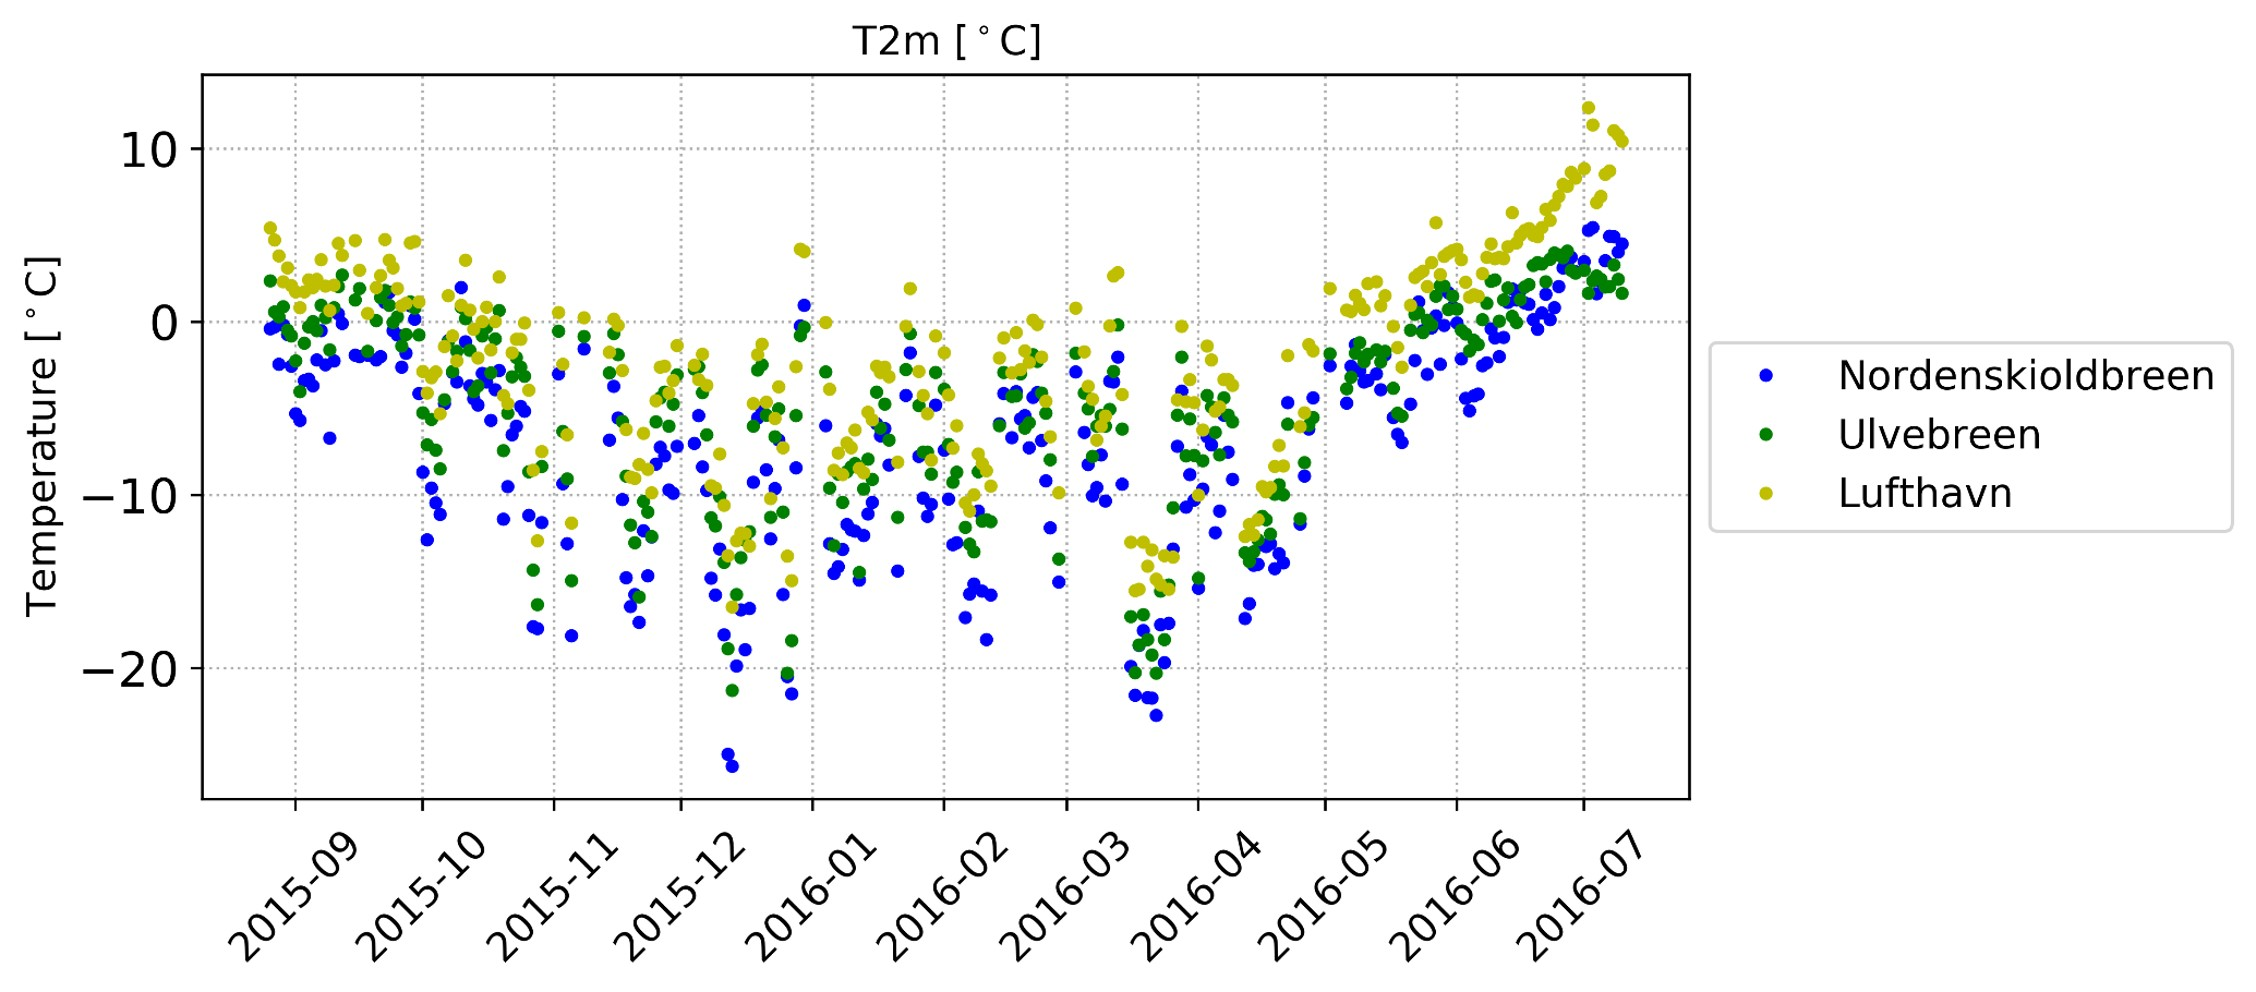
\includegraphics[scale=1, width=1\textwidth]{T2m.jpg}
    \label{fig:T2m}
    \caption{Comparison of temperature at 2 meter height for Nordenski\H{o}ldbreen, Ulvebreen and Lufthavn, where colors are corresponding to the legend.}
\end{figure}

Also, the surface temperature of both glaciers Nordenski\H{o}ldbreen and Ulvebreen are compared with each other, visible in figure 
\ref{fig:Tsurf}. Looking through the different values at the axis, the Nordenski\H{o}ldbreen looks colder. To correct for this, again the lapse rate is used of 2,334 degrees (from equation \ref{eq:lr}) which is added to the data, corresponding to the black line in figure \ref{fig:Tsurf}. For example, when a temperature of -10 degrees Celcius is reached at the Ulvebreen, it has to be -12,3 degrees at Nordenski\H{o}ldbreen when corrected for height. With this lapse rate, it is 0.15 degrees Celcius warmer at the Ulvebreen than expected. Again, a T-test is done for the difference in surface temperatures for both glaciers. With a p-value of 0.7, the Ulvebreen is not significant warmer than the Nordenski\H{o}ldbreen.

To conclude, taking into account the lapse rate, the temperatures overlap really well. So, the temperature differences between the locations of the measurement are related to the height of the measurements.

%0.148485162556455  degrees Celsius colder in Ulvebreen than expected from lapse rate
%p is Ttest_indResult(statistic=-0.3463400286433108, pvalue=0.7291681410617556)

\begin{figure}[h]
\centering{}
    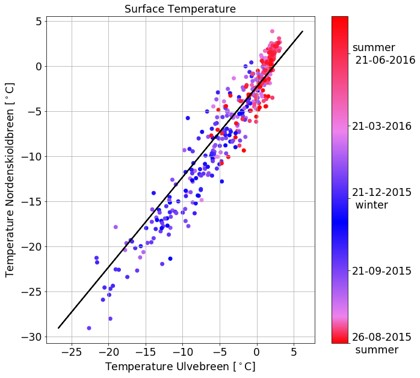
\includegraphics[scale=0.5, width=0.5\textwidth]{Tsurf.jpg}
    \label{fig:Tsurf}
    \caption{Comparison of surface temperature of Ulvebreen, visible at the x-axis and the Nordenski\H{o}ldbreen, visible at the y-axis. In colors, the dates are visible from summer 2015 in red below, via winter 2015 in blue, to summer 2016 above, again in red. For explanation of the black line, see text.}
\end{figure}

\newpage
However, also visible in figure \ref{fig:Tsurf} are the temperatures which are slightly above 0 degrees for both glaciers. This is not expected, because at a value of 0 degrees, the ice will melt and the energy will be converted. To investigate this furthermore, the incoming shortwave radiation is compared with the wind speed and hut temperature for the Nordenski\H{o}ldbreen. For this, all years of data of the Nordenski\H{o}ldbreen is used between 21 June and 21 September. This is plotted in figure \ref{fig:Thut}. If the sensor is influenced by the wind speed, we expected a higher temperature of the hut at a lower wind speed and a high incoming surface radiation. Unfortunately, no clearly relation is visible. With this, we can conclude that the sensors of surface temperature of both glaciers do probably have a short standard deviation. 

\begin{figure}[h]
\centering{}
    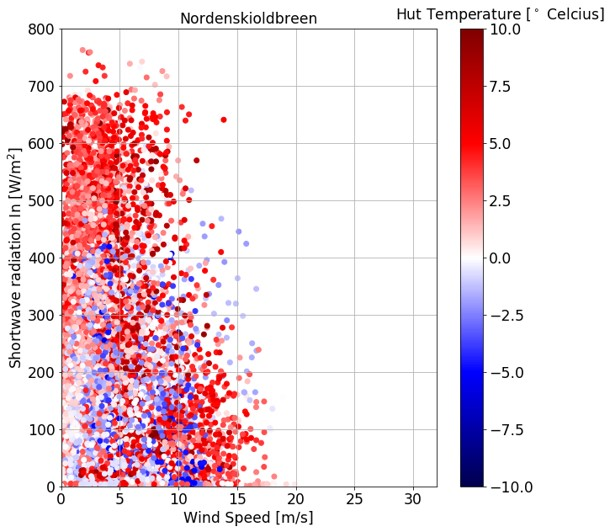
\includegraphics[scale=0.5, width=0.5\textwidth]{Thut-Sin.jpg}
    \label{fig:Thut}
    \caption{Comparison of the wind speed at the x-axis, the incoming shortwave radiation at the y-axis and the hut temperature corresponding to the colorbar at Nordenski\H{o}ldbreen for all available years between 21 June and 21 September (summer) }
\end{figure}


\newpage
\section{Prevailing winds}\label{sec:katw}
Next to the temperatures of the glaciers, the differences in wind direction and wind speed are investigated. This is done for both glaciers apart, to take all data points of each glacier into account. Results are visible in the plots in figure \ref{fig:PR}. 

\begin{figure}[h]
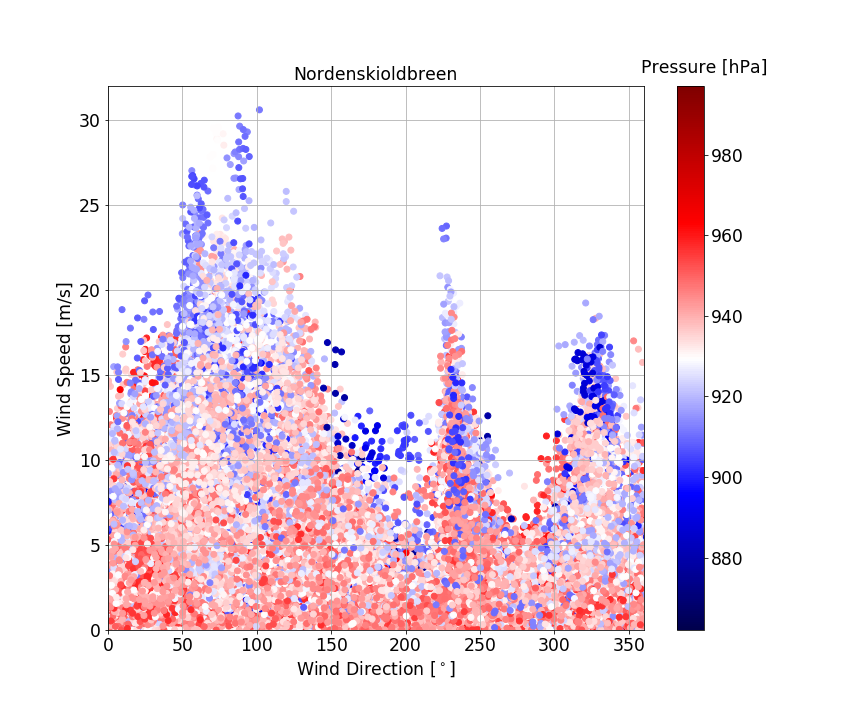
\includegraphics[scale=1, width=0.5\textwidth]{WD-WS-PR-Nordenskioldbreen.png}
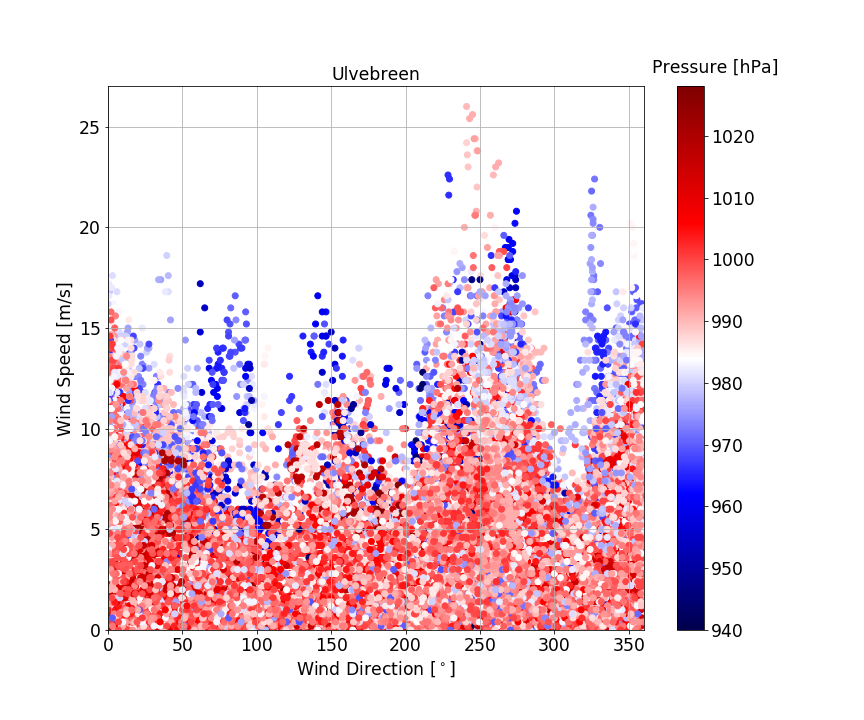
\includegraphics[scale=1, width=0.5\textwidth]{WD-WS-PR-Ulvebreen.png}
\caption{Comparison of the wind direction at x-axis, wind speed at y-axis and the corresponding pressure, related to the colorbar. Left: Nordenski\H{o}ldbreen and right: Ulvebreen}
\label{fig:PR}
\end{figure}

Within these plots, katabatic winds are clearly visible at the Ulvebreen at 250 degrees. Comparing this again to the map in figure \ref{fig:ulve}, direction is visible.


%suggesties:
%valley glacier?
%breedte glacier vs tunneling effect?
%Schaduw van eigen sensor?
%vergelijken wolkenvrije dagen versus schaduw versus windrichting
%schaduwwerking sensor
%topografie
%ra ging kapot dus los van mast?
%zomermaanden water, vries vast in winter


%a wind that carries high-density air from a higher elevation down a slope under the force of gravity.

Usually the higher the wind speed, the lower the pressure, but an exception is visible for the katabatic wind speed. Thereby around 
Nordeskioldbreen 50 graden met een breder spectrum, omdat uit verschillende hoeken wind mogelijk. 



\begin{figure}[h]
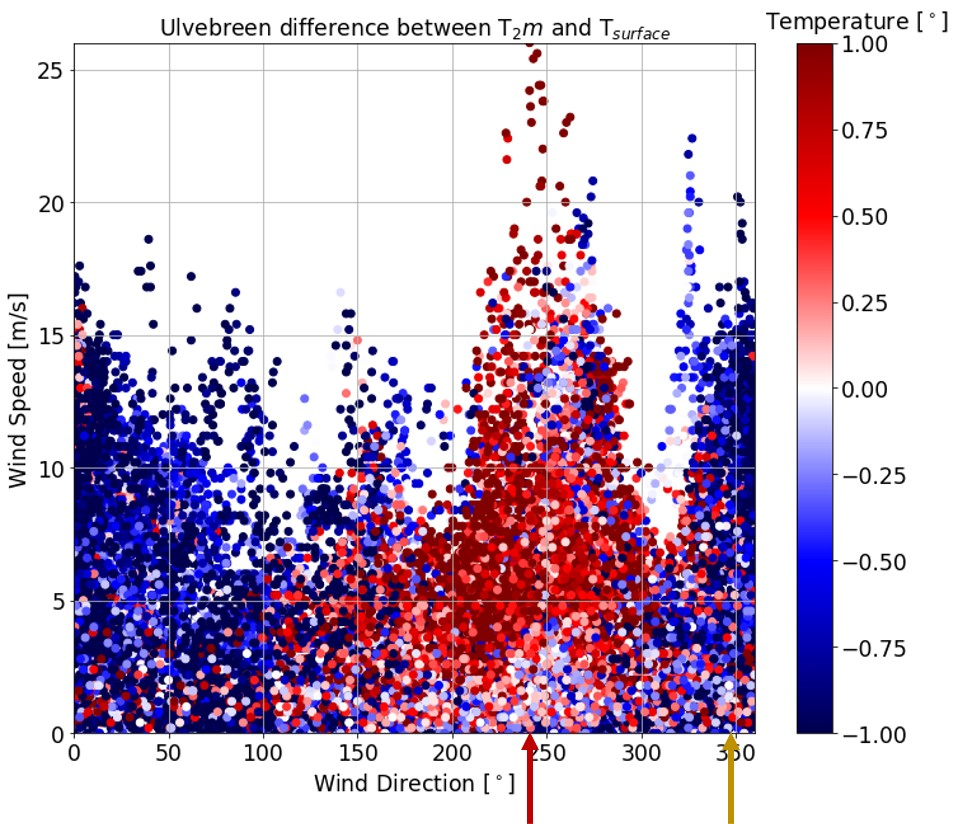
\includegraphics[scale=1, width=0.55\textwidth]{norde-WS-WD.jpg}
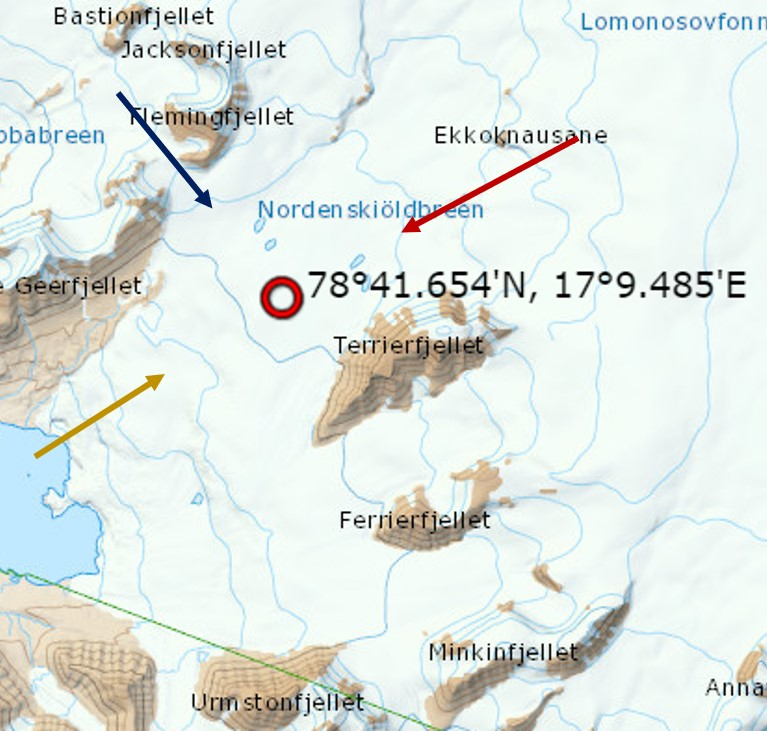
\includegraphics[scale=1, width=0.45\textwidth]{norde-WS-WD-rose-2.jpg}
\caption{Left: Comparison of the wind direction at x-axis, wind speed at y-axis and the corresponding pressure, related to the colorbar. Right: Maps with wind directions, related to colors left.}
\label{fig:PRnorde}
\end{figure}

\begin{figure}[h]
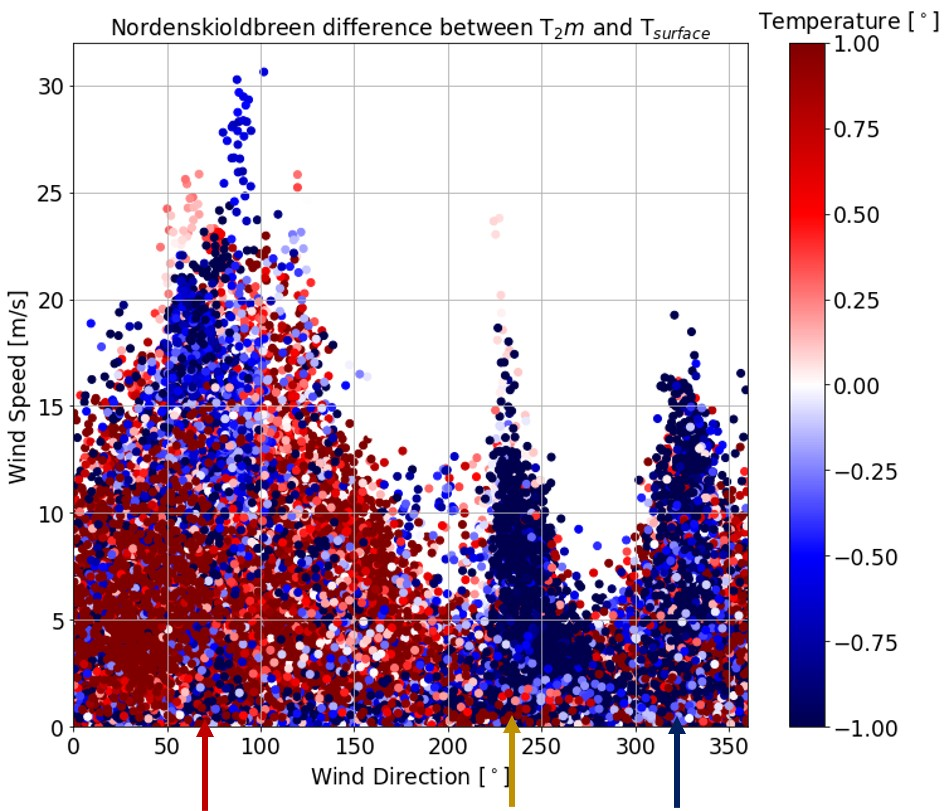
\includegraphics[scale=1, width=0.55\textwidth]{ulve-WS-WD.jpg}
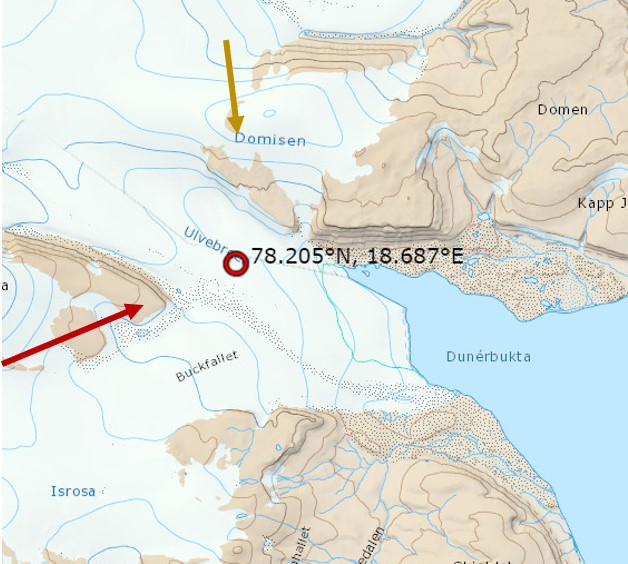
\includegraphics[scale=1, width=0.45\textwidth]{ulve-WS-WD-rose-1.jpg}
\caption{Left: Comparison of the wind direction at x-axis, wind speed at y-axis and the corresponding pressure, related to the colorbar. Right: Maps with wind directions, related to colors left.}
\label{fig:PRulve}
\end{figure}


\newpage
\section{Radiation, snow height, albedo}\label{sec:rad}
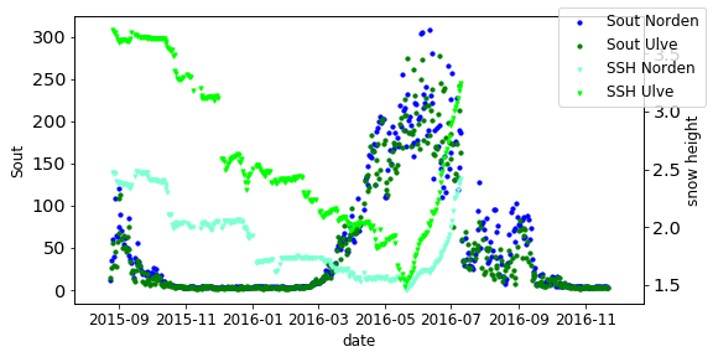
\includegraphics[scale=1, width=0.35\textwidth]{Picture1.jpg}
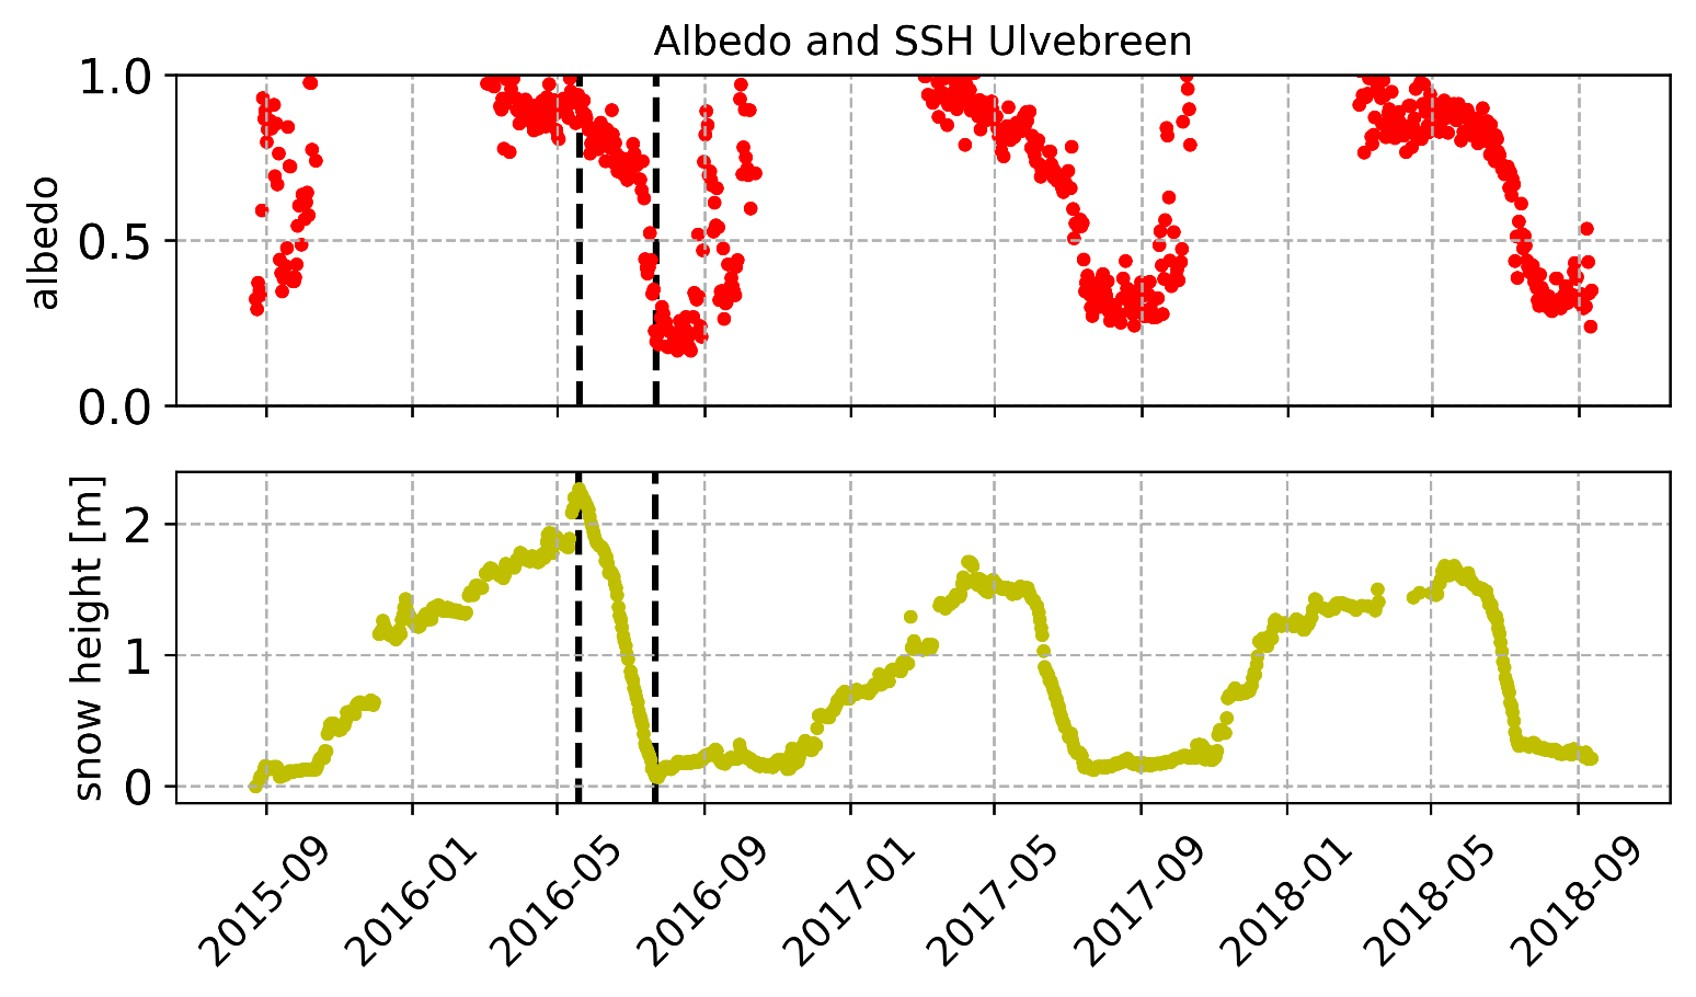
\includegraphics[scale=1, width=0.35\textwidth]{Picture2.jpg}


\chapter{Discussion}\label{sec:discussion}
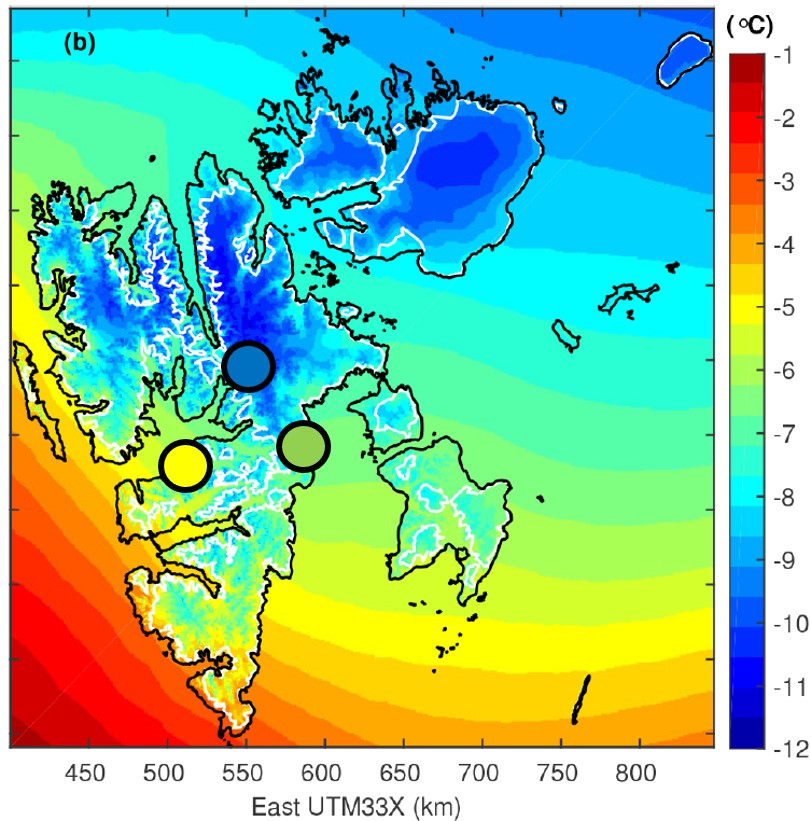
\includegraphics[scale=1, width=0.35\textwidth]{ostby.jpg}
\cite{osby}





\chapter{Conclusion}\label{sec:conclusion}

\textcolor{red}{
Temperatures are highly dependend on location of latitude and longitue and height\\
direction glacier related to Wind direction and katabatic wind\\
differences in albedo related to different Sin in time and amount, dirty snow/ice}

\chapter{Recommandations}\label{sec:rec}
"Vijf jaar na de succesvolle eerste SEES.NL expeditie, willen we graag weer terug om de veranderingen vast te leggen. Het concept is net als in 2015. Allerlei wetenschappers aangevuld met toeristen. We hebben hulp nodig om dit mogelijk te maken. Geef je vrijblijvend op als wetenschapper, toerist of sponsor. Dan nemen we snel contact met je op."
\medskip

\begin{thebibliography}{9}
\addcontentsline{toc}{chapter}{Bibliography}
\bibitem{sval}
Website: The University Centre in Svalbard, UNIS (01-2018), 
\textit{The Early Exploration of the Arctic and the Discovery of
Svalbard},
Retrieved at 30-10-2018, from:\\
\texttt{\small{https://www.unis.no/wp-content/uploads/2018/01/SH201\_Summary02\_2018.pdf}}

\bibitem{sees}
Website: Netherlands Scientific Expedition Edgeøya Spitsbergen, SEES, (2015), \\ Retrieved at 30-10-2018, from:
\texttt{\small{http://www.sees.nl/}}\\

\bibitem{abl}
Article: Hulth, J. (2010). 
\textit{Using a draw-wire sensor to continuously monitor glacier melt.} Journal of Glaciology, 56(199), 922-924. 
\texttt{doi:10.3189/002214310794457290}

\bibitem{uuproj}
Website: Institute for Marine and Atmospheric Research (IMAU)
\textit{Ice and Climate: Automatic Weather Stations on glaciers}
Retrieved at 30-10-2018, from:
\texttt{https://www.projects.science.uu.nl/iceclimate/aws/files\_oper/}

\bibitem{1}
Website: Norwegian Meteorological Institute Svalbard climate data
\textit{Weather statistics for Longyearbyen (Svalbard)},
Retrieved at 30-10-2018, from:
\texttt{https://www.yr.no/place/Norway/Svalbard/Longyearbyen/statistics.html}


\bibitem{2}
Article: Storrie, Luke, Lydersen, Christian, Andersen, Magnus, B.Wynn, Russell and Kovacs, Kit. (2018). 
\textit{Determining the species assemblage and habitat use of cetaceans in the Svalbard Archipelago, based on observations from 2002 to 2014.} Polar Research. 37. 10.1080/17518369.2018.1463065. 

\bibitem{sharkii}
Website: eKlima \textit{the climate database of the Norwegian Meteorological Institute}, Retrieved at 30-10-2018, from:
\texttt{http://sharki.oslo.dnmi.no/}

\bibitem{osby}
Article: Østby, T. I., Schuler, T. V., Hagen, J. O., Hock, R., Kohler, J., and Reijmer, C. H.: \texttt{Diagnosing the decline in climatic mass balance of glaciers in Svalbard over 1957–2014}, 
The Cryosphere, 11, 191-215 \texttt{https://doi.org/10.5194/tc-11-191-2017}, 2017.

\end{thebibliography}

%\chapter*{Appendices}
%\addcontentsline{toc}{chapter}{Appendices}

%\section*{A. name}\label{Ap:A}
%\setcounter{figure}{0}
%\renewcommand{\thefigure}{A.\arabic{figure}}
%\addcontentsline{toc}{section}{A. name}



\end{document}
